\documentclass[10pt, a4paper]{article}

% --- Gói cần thiết ---
\usepackage[utf8]{inputenc}
\usepackage[T5]{fontenc} % Dành cho tiếng Việt (mặc dù nội dung này là tiếng Anh, nhưng chuẩn bị sẵn)
\usepackage{float}
\usepackage{amsmath}
\usepackage{amssymb}
\usepackage{graphicx}
\usepackage{hyperref} % Dùng cho các siêu liên kết trong tài liệu và URL
\usepackage{booktabs} % Để tạo bảng chuyên nghiệp hơn (dùng \toprule, \midrule, \bottomrule)
\usepackage{geometry} % Để căn lề
\usepackage{authblk} % Để định dạng tên tác giả
\usepackage{abstract} % Để tùy chỉnh tiêu đề Abstract
\usepackage{tikz} 
\usetikzlibrary{shapes, arrows.meta, positioning, fit, backgrounds, calc}
\usepackage{tabularx}
\usepackage{pgfplots}
\pgfplotsset{compat=1.17}
% --- Thiết lập Geometry (Căn lề) ---
\geometry{
    a4paper,
    top=1in,
    bottom=1in,
    left=1in,
    right=1in,
    hmarginratio={1:1},
    vmarginratio={1:1},
    landscape,
    margin=1in
}

% --- Tùy chỉnh Tiêu đề và Abstract ---
\renewcommand{\abstractname}{ABSTRACT}
\setlength{\absleftindent}{0.0in}
\setlength{\absrightindent}{0.0in}
\renewcommand{\Affilfont}{\itshape\small}

% --- Bắt đầu tài liệu ---
\begin{document}

\title{\textbf{Solidify: Real-Time Static Analysis for Solidity in IDE}}
\author{Nguyen Huu Canh, Sit Khai Dong}
\date{November 30, 2025}
\maketitle

\section*{ABSTRACT}
Smart contracts underpin decentralized finance (DeFi) and Web3 applications, stewarding billions of dollars in value. Security defects in Solidity code can cause catastrophic losses. Existing static analyzers are typically wired into continuous integration (CI/CD) pipelines and surface findings only after code is written, leaving a blind spot during development when issues could be caught immediately.

This paper introduces \textbf{Solidify}, a Visual Studio Code extension that delivers real-time static analysis directly inside the integrated development environment (IDE). The tool adopts a hybrid strategy: it leverages \texttt{tree-sitter} to construct rich Abstract Syntax Trees (ASTs) while complementing them with high-performance regular expressions for rapid pattern checks. A modular rule architecture makes it straightforward to extend coverage across security, syntax, naming conventions, and pragma versioning.

Our evaluation on 20 real-world smart contracts shows that Solidify achieves an average analysis latency of 82 ms ($\pm$ 15 ms), roughly 30$\times$ faster than baseline tools such as Slither ($\sim 2.5$ s). The analyzer attains $F1 = 0.60$ (Precision: 0.61, Recall: 0.59), demonstrating that sacrificing some depth of analysis for instant feedback is both practical and impactful for developer experience.

\textbf{Index Terms:} Smart Contracts, Solidity, Static Analysis, Blockchain Security, Visual Studio Code, Abstract Syntax Tree (AST).

\section*{INTRODUCTION}
The rise of blockchain technology ushered in a new era of decentralized applications with smart contracts at the core. Solidity has become the de facto language for authoring these contracts on Ethereum and other EVM-compatible chains. Yet the immutability of blockchain - the very property that ensures trust-cuts both ways: once deployed, smart contract code cannot be patched. Seemingly minor vulnerabilities can be exploited to drain digital assets worth millions of dollars [1].

High-profile incidents such as The DAO (2016) or the Parity Wallet hack (2017) underscore the need for rigorous code inspection. The community responded with heavyweight static analyzers like Slither [2] and Mythril [3]. These tools excel at deep analysis but are optimized for whole-project scans, often within CI/CD pipelines. Developers therefore receive feedback only after finishing significant work and pushing their changes. This slow feedback loop raises the cost of fixes and hampers productivity.

We identify a critical gap: the lack of tools that raise security and syntax warnings while a developer is typing. Immediate feedback not only accelerates remediation but also reinforces best practices by highlighting anti-patterns in context.

To close this gap we built \textbf{Solidify}, a VS Code extension designed to be lightweight, responsive, and tightly integrated with the editor, effectively acting as a real-time assistant for Solidity developers.

Our main contributions are:
\begin{itemize}
    \item \textbf{Hybrid analysis architecture:} We present a design that combines AST-based reasoning with regex-based pattern detection.
    \item \textbf{Modular rule system:} We architect the analyzer so that rules can be developed, maintained, and extended independently.
    \item \textbf{Real-time integration:} We implement an IDE-native static analyzer that produces instant feedback without disrupting the developer’s flow.
    \item \textbf{Comprehensive rule set:} We deliver an initial suite that addresses high-impact security flaws, common syntax mistakes, and code quality conventions.
\end{itemize}

\section*{RELATED WORK}
Security analysis of smart contracts has attracted significant research. Existing tools broadly fall into static or dynamic analysis categories.

\textbf{Static analysis} inspects source code without execution. \textbf{Slither} [2] is among the most capable frameworks, operating on its SlithIR intermediate representation to detect a wide range of vulnerabilities. \textbf{Mythril} [3] performs symbolic execution to explore attackable states. \textbf{Securify} [4] employs dependency patterns to verify contract correctness. Despite their power, these tools are heavy, require lengthy analysis times, and are not designed for instantaneous IDE feedback.

\textbf{Dynamic analysis} executes contracts in controlled environments to observe behavior. Tools like Manticore [5] can traverse complex execution paths but at considerable computational cost.

Popular IDE extensions, such as Juan Blanco’s Solidity extension [6], offer features like code completion, formatting, and compilation, yet provide limited real-time security diagnostics.

Solidify aims to bridge the gap between deep static analyzers and lightweight IDE tooling. The goal is not to replace Slither in CI/CD pipelines, but to supply a first line of defense that continuously shifts security detection to the left in the development lifecycle.

\begin{table}[h]
    \centering
    \caption{Comparison of Existing Smart Contract Analysis Tools vs. Solidify}
    \label{tab:related_work_comparison}
    \begin{tabularx}{\textwidth}{@{} l >{\raggedright\arraybackslash}X c c c @{}}
        \toprule
        \textbf{Tool} & \textbf{Analysis Method} & \textbf{Speed} & \textbf{Environment} & \textbf{Real-time Feedback} \\
        \midrule
        Slither & Static (SlithIR) & Slow & CI/CD & No \\
        Mythril & Symbolic Execution & Slow & CI/CD & No \\
        Securify & Dependency Patterns & Slow & CI/CD & No \\
        Manticore & Dynamic Analysis & Very Slow & Testing Env. & No \\
        Standard IDE Ext. & Syntax Checking & Fast & IDE & Limited \\
        \midrule
        \textbf{Solidify} & \textbf{Hybrid (AST + Regex)} & \textbf{Instant} & \textbf{IDE} & \textbf{Yes} \\
        \bottomrule
    \end{tabularx}
\end{table}

\section*{METHODOLOGY}
Meeting real-time performance targets while maintaining accuracy requires a hybrid and modular design.

\subsection*{Hybrid Analysis Architecture}
Solidify blends two complementary analysis techniques:
\begin{enumerate}
    \item \textbf{AST-based analysis:} We rely on the \texttt{tree-sitter} library [7] and the \texttt{tree-sitter-solidity} grammar to parse source code into an AST. \texttt{tree-sitter} is fast, incremental, and resilient to incomplete or syntactically invalid code-critical properties for real-time tooling. ASTs reveal structural and semantic information such as:
    \begin{itemize}
        \item Determining variable scope to flag declarations that are never used.
        \item Differentiating variable declarations from references.
        \item Locating function bodies and control structures for rule evaluation.
    \end{itemize}
    \item \textbf{Regex-based analysis:} Traversing the AST for every lightweight rule can be overkill. For localized patterns, regular expressions are faster. We use regex for tasks like:
    \begin{itemize}
        \item Detecting dangerous or deprecated keywords (\texttt{tx.origin}, \texttt{suicide}).
        \item Enforcing naming conventions.
        \item Spotting simple syntax mistakes, such as missing semicolons.
    \end{itemize}
\end{enumerate}
This hybrid approach leverages regex speed for simple checks and AST precision for context-aware rules.

\subsection*{System Architecture}
Solidify follows a five-layer architecture in which each layer builds upon services provided by the one beneath it, isolating responsibilities and easing long-term maintenance:
\begin{itemize}
    \item \textbf{Layer 1 - VS Code Integration:} The outer layer anchors the tool to the IDE lifecycle. It registers \texttt{TextDocument} listeners, manages activation/disposal, and provides debounce mechanisms when users type rapidly. This is the sole entry point to VS Code APIs.
    \item \textbf{Layer 2 - Core Analysis Engine:} The coordinator receives requests from Layer 1, normalizes inputs, manages caches, and orchestrates the analysis pipeline. It defines shared interfaces such as \texttt{RuleContext} and \texttt{RuleFinding} for upper layers.
    \item \textbf{Layer 3 - AST/CFG Processing:} This middle layer constructs structural views of the contract. Solidify invokes \texttt{tree-sitter} to build ASTs and infers basic control relationships (function boundaries, conditional blocks, loops) to emulate a lightweight control-flow graph (CFG). The resulting context objects allow rules to consume structured data without traversing the tree directly.
    \item \textbf{Layer 4 - Enhanced Rules Engine:} The modules that define the rules are resided here, each dedicated to a domain. With consistent interfaces from Layer 2 and context from Layer 3, rule authors focus on detection logic rather than infrastructure.
    \item \textbf{Layer 5 - Advanced Diagnostic Display:} The presentation layer converts findings into \texttt{DiagnosticCollection} entries, assigns severities, formats messages, and surfaces highlights, popovers, and the Problems panel. It is also the hook for future features like Quick Fixes or telemetry.
\end{itemize}
This layered architecture isolates change: adding rules affects Layer 4, optimizing AST/CFG logic touches Layer 3, while IDE integration remains stable in Layer 1.

\begin{figure}[H]
    \centering
    \resizebox{\textwidth}{!}{% Tự động co giãn sơ đồ cho vừa trang giấy
    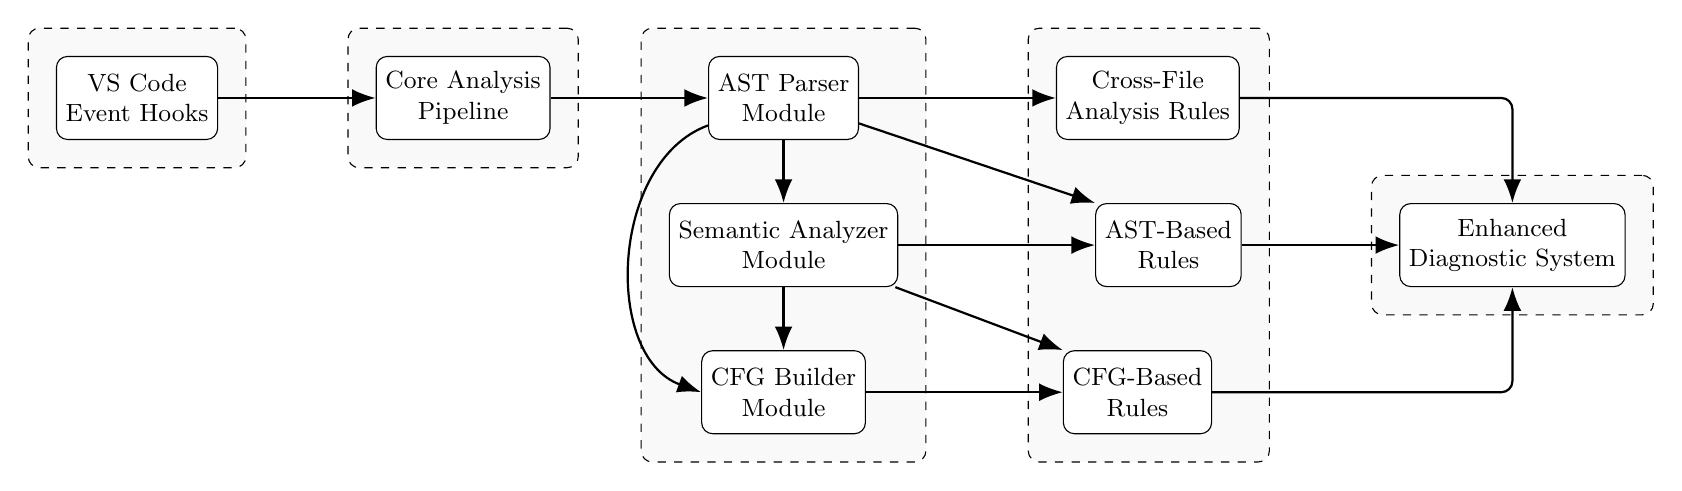
\begin{tikzpicture}[
        % Định nghĩa kiểu dáng (Style) cho các khối
        node distance=1.5cm and 1cm, % Khoảng cách giữa các khối (dọc và ngang)
        block/.style={
            rectangle, 
            draw, 
            rounded corners, 
            minimum height=3em, 
            minimum width=4em, 
            text centered, 
            align=center, 
            fill=white,
            font=\small
        },
        group/.style={
            draw, 
            dashed, 
            inner sep=10pt, 
            rounded corners, 
            fill=gray!5
        },
        arrow/.style={
            -{Latex[length=3mm]}, 
            thick,
            rounded corners
        },
        label_text/.style={
            anchor=north west,
            font=\bfseries\small,
            yshift=-2pt
        }
    ]

    % --- 1. VẼ CÁC NODE (KHỐI) ---
    
    % L1: VS Code Integration
    \node[block] (ext) {VS Code\\Event Hooks};

    % L2: Core Analysis Engine (Nằm bên phải L1)
    \node[block, right=2cm of ext] (core) {Core Analysis\\Pipeline};

    % L3: AST/CFG Processing (Nằm bên phải L2)
    % Sắp xếp dọc: Parser trên cùng, Semantic giữa, CFG dưới
    \node[block, right=2cm of core] (parser) {AST Parser\\Module};
    \node[block, below=0.8cm of parser] (semantic) {Semantic Analyzer\\Module};
    \node[block, below=0.8cm of semantic] (cfg) {CFG Builder\\Module};

    % L4: Enhanced Rules Engine (Nằm bên phải L3)
    % Sắp xếp tương ứng để đường nối đẹp nhất
    \node[block, right=2.5cm of parser] (crossFile) {Cross-File\\Analysis Rules};
    \node[block, right=2.5cm of semantic] (astRule) {AST-Based\\Rules};
    \node[block, right=2.5cm of cfg] (cfgRule) {CFG-Based\\Rules};

    % L5: Advanced Diagnostic Display (Nằm bên phải L4)
    % Đặt ở giữa theo chiều dọc so với nhóm L4
    \node[block, right=2cm of astRule] (diag) {Enhanced\\Diagnostic System};

    % --- 2. VẼ CÁC ĐƯỜNG NỐI (EDGES) ---
    
    % L1 -> L2
    \draw[arrow] (ext) -- (core);

    % L2 -> L3
    \draw[arrow] (core) -- (parser);

    % Nội bộ L3
    \draw[arrow] (parser) -- (semantic);
    \draw[arrow] (parser) to[out=200,in=160] (cfg.west); % Đường cong nhẹ để tránh chồng lấn
    \draw[arrow] (semantic) -- (cfg);

    % L3 -> L4
    \draw[arrow] (parser) -- (crossFile);
    \draw[arrow] (parser) -- (astRule.north west);
    \draw[arrow] (semantic) -- (astRule);
    \draw[arrow] (semantic) -- (cfgRule.north west);
    \draw[arrow] (cfg) -- (cfgRule);

    % L4 -> L5
    \draw[arrow] (crossFile) -| (diag); % Đường vuông góc
    \draw[arrow] (astRule) -- (diag);
    \draw[arrow] (cfgRule) -| (diag);   % Đường vuông góc

    % --- 3. VẼ SUBGRAPH (BACKGROUND LAYER) ---
    % Sử dụng thư viện 'backgrounds' để vẽ các khung phía sau node
    \begin{scope}[on background layer]
        % L1 Frame
        \node[group, fit=(ext)] (l1) {};
        \node[label_text] at (l1.north west) {};

        % L2 Frame
        \node[group, fit=(core)] (l2) {};
        \node[label_text] at (l2.north west) {};

        % L3 Frame
        \node[group, fit=(parser) (semantic) (cfg)] (l3) {};
        \node[label_text] at (l3.north west) {};

        % L4 Frame
        \node[group, fit=(crossFile) (astRule) (cfgRule)] (l4) {};
        \node[label_text] at (l4.north west) {};

        % L5 Frame
        \node[group, fit=(diag)] (l5) {};
        \node[label_text] at (l5.north west) {};
    \end{scope}

    \end{tikzpicture}
    } % End resizebox
    \caption{Solidify System Architecture}
    \label{fig:architecture}
\end{figure}

\section*{RESULTS}
We assess Solidify along two axes: performance, measured by analysis latency, and accuracy, measured by standard security metrics (Precision, Recall, F1-Score).

\subsection*{Experimental Setup.}
Dataset: We collect 20 real-world Solidity smart contracts of varying size and complexity. Contracts are sampled from popular open-source projects on GitHub to ensure diversity and relevance.

Baseline Tool: Slither serves as the baseline given its prominence and state-of-the-art status in Ethereum contract analysis.

Hardware Configuration: All experiments run on identical hardware (CPU: Intel i9-14900HX, RAM: 32 GB) to guarantee fair comparison.

\begin{table}[H]
    \centering
    \caption{Comparison of Solidify vs. Slither Performance and Accuracy}
    \label{tab:comparison}
    
    % Sử dụng tabularx và đặt chiều rộng là \textwidth (bằng chiều rộng văn bản)
    % Cấu trúc cột: 
    % X: Cột đầu tiên tự động giãn (mặc định canh trái)
    % >{\centering\arraybackslash}X: Các cột sau cũng tự giãn nhưng canh giữa
    \begin{tabularx}{\textwidth}{@{} X >{\centering\arraybackslash}X >{\centering\arraybackslash}X @{}}
        \toprule
        \textbf{Metric} & \textbf{Solidify} & \textbf{Slither} \\
        \midrule
        Analysis Latency & 82ms ($\pm$ 15ms) & $\sim$ 2.5s \\
        \midrule
        Precision & 0.61 & 0.91 \\
        \midrule
        Recall & 0.59 & 0.94 \\
        \midrule
        F1 Score & 0.60 & 0.92 \\
        \midrule
        False Positives & 0.39 & 0.09 \\
        \bottomrule
    \end{tabularx}
\end{table}

\subsection*{Response Latency.}
The primary goal of Solidify is instantaneous feedback. We compare average analysis latency against Slither.

Solidify reaches 82 ms on average, well below the sub-100 ms human-interaction threshold. This is roughly 30$\times$ faster than Slither ($\sim 2.5$ s), illustrating our core contribution: transforming static analysis from a slow CI/CD batch step into an immediate IDE experience.

\begin{figure}[H]
    \centering
    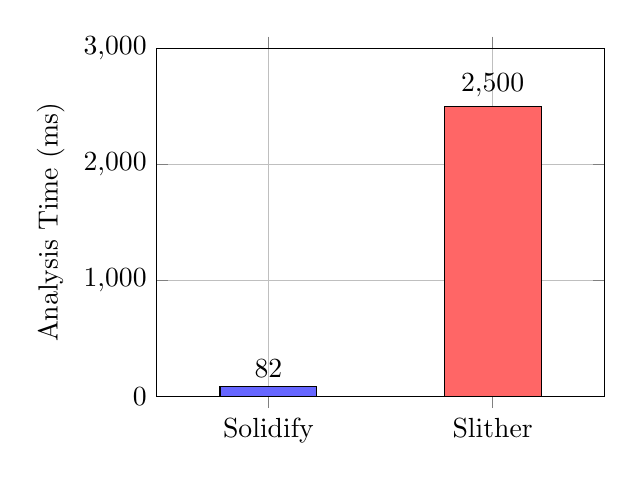
\begin{tikzpicture}
        \begin{axis}[
            ybar,
            bar width=35pt,
            width=0.6\textwidth,
            height=6cm,
            enlarge x limits=0.5,
            symbolic x coords={Solidify, Slither},
            xtick={Solidify, Slither}, 
            ylabel={Analysis Time (ms)},
            ymin=0, 
            ymax=3000,
            grid=major,
            nodes near coords,
            every node near coords/.append style={font=\bfseries},
            bar shift=0pt 
        ]
        % Cột Solidify (Màu Xanh)
        \addplot[fill=blue!60, draw=black] coordinates {
            (Solidify, 82)
        };
        % Cột Slither (Màu Đỏ)
        \addplot[fill=red!60, draw=black] coordinates {
            (Slither, 2500)
        };
        \end{axis}
    \end{tikzpicture}
    \caption{Average Analysis Latency Comparison}
    \label{fig:latency_comparison}
\end{figure}

\subsection*{Accuracy Metrics.}
We evaluate detection quality of Solidify versus Slither on the same dataset.

Slither secures a much higher F1 score (0.92 vs. 0.60). Its whole-program analysis yields rich control-flow graphs and sophisticated data-flow analyses that suppress false positives. In contrast, Solidify favors hybrid AST/regex techniques geared for speed, accepting higher noise (Precision: 0.61, False Positives: 39\%) in exchange for immediate responsiveness.

\begin{figure}[H]
    \centering
    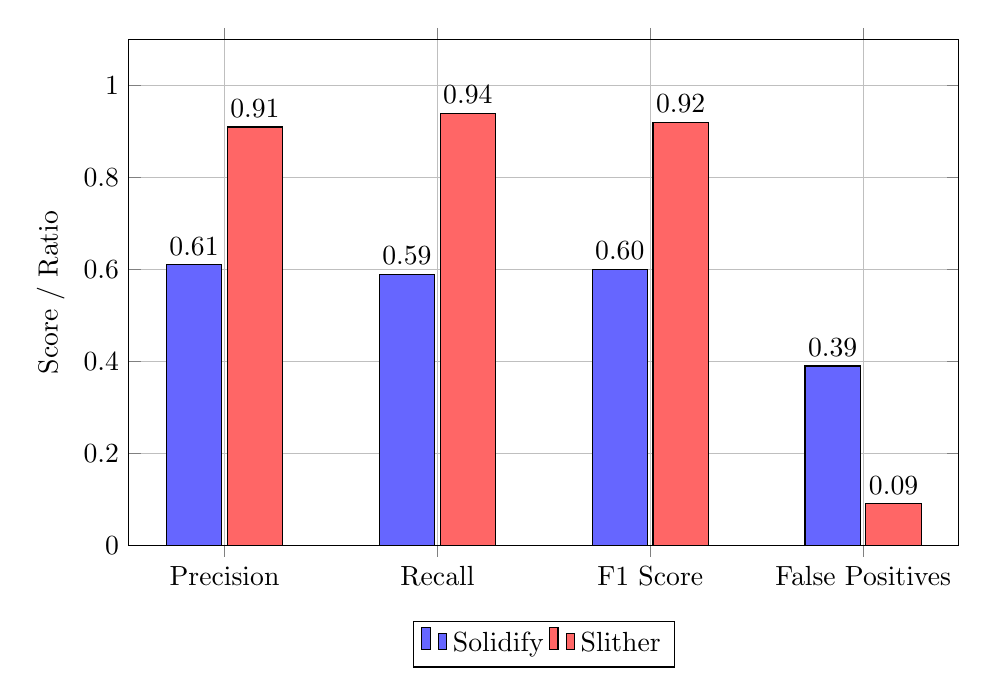
\begin{tikzpicture}
        \begin{axis}[
            ybar,
            bar width=20pt,
            width=\textwidth,
            height=8cm,
            enlarge x limits=0.15,
            symbolic x coords={Precision, Recall, F1 Score, False Positives},
            xtick=data,
            ymin=0, ymax=1.1,
            ylabel={Score / Ratio},
            grid=major,
            nodes near coords={\pgfmathprintnumber[fixed, fixed zerofill, precision=2]{\pgfplotspointmeta}},
            every node near coords/.append style={font=\footnotesize},
            legend style={at={(0.5,-0.15)}, anchor=north, legend columns=-1}
        ]
        
        % Dữ liệu của Solidify (Xanh)
        \addplot[fill=blue!60, draw=black] coordinates {
            (Precision,0.61) 
            (Recall,0.59) 
            (F1 Score,0.60) 
            (False Positives,0.39)
        };
        
        % Dữ liệu của Slither (Đỏ)
        \addplot[fill=red!60, draw=black] coordinates {
            (Precision,0.91) 
            (Recall,0.94) 
            (F1 Score,0.92) 
            (False Positives,0.09)
        };
        
        \legend{Solidify, Slither}
        \end{axis}
    \end{tikzpicture}
    \caption{Comparative Analysis of Accuracy Metrics between Solidify and Slither}
    \label{fig:accuracy_comparison}
\end{figure}

\section*{DISCUSSION}
\textbf{Solidify} proves effective as a “first-line defense.” Deep IDE integration shifts security feedback from a deferred activity to a continuous part of editing.

\subsection*{Strengths.}
The latency advantage stems from lightweight, scope-aware analysis and high-speed \texttt{tree-sitter} parsing, whereas Slither must build SlithIR and execute heavier analyses.

The lower accuracy (F1 = 0.60 vs. 0.92) is an intentional trade-off. Slither’s whole-program reasoning exposes complex vulnerabilities (e.g., multi-contract reentrancy). Solidify, in contrast, concentrates on syntax mistakes, local anti-patterns, and straightforward security hazards where instant feedback matters most. Our goal is to reduce developer-facing false positives early, not to supplant deep audits.

\subsection*{Limitations.}
Solidify is not designed for cross-contract analysis or symbolic execution. It catches common, localized issues but cannot replace comprehensive project-wide analyses or formal audits. We recommend using Solidify alongside heavyweight tooling in CI/CD and traditional security reviews.

\section*{CONCLUSION}
We presented Solidify, a real-time static analysis extension for Solidity inside VS Code. By combining AST reasoning and regex heuristics, we markedly shorten the feedback loop for developers. Experiments show 82 ms latency-30$\times$ faster than CI/CD-oriented analyzers-while maintaining $F1 = 0.60$. This demonstrates the viability of trading analytical depth for speed to enhance developer experience and promote secure coding habits from the outset.

Future work includes:
\begin{itemize}
    \item \textbf{Advanced rules:} Detect more sophisticated patterns such as reentrancy, integer overflow/underflow (with compiler assistance), and unsafe delegation flows.
    \item \textbf{Quick Fix integration:} Offer automated fixes, e.g., adding \texttt{payable} or removing unused variables.
    \item \textbf{Configurability:} Allow developers to tune severities or suppress specific diagnostics inline.
    \item \textbf{Performance research:} Further optimize analysis algorithms and introduce caching for very large projects.
    \item \textbf{Deeper analysis:} Incorporate selected intra-function data-flow analyses to curb false positives.
\end{itemize}
Empowering developers with intelligent, integrated, and instantaneous tooling is crucial to building a safer, more trustworthy Web3 ecosystem.

\renewcommand{\refname}{REFERENCES}
\begin{thebibliography}{9}
\bibitem{1} N. Atzei, M. Bartoletti, and T. Cimoli, “A survey of attacks on Ethereum smart contracts,” in \textit{Principles of Security and Trust (POST)}, ser. Lecture Notes in Computer Science, vol. 10260. Cham: Springer, 2017, pp. 109–139.
\bibitem{2} J. Feist, G. Grieco, and G. Mvel, “Slither: A static analysis framework for smart contracts,” in \textit{IEEE International Conference on Blockchain (Blockchain)}, 2019, pp. 1–9.
\bibitem{3} B. Mueller, “Mythril: A security analysis tool for Ethereum smart contracts,” GitHub repository. [Online]. Available: \url{https://github.com/ConsenSysDiligence/mythril}
\bibitem{4} P. Tsankov et al., “Securify: Practical security analysis of smart contracts,” in \textit{Proceedings of the 2018 ACM SIGSAC Conference on Computer and Communications Security (CCS)}, 2018, pp. 673–688.
\bibitem{5} M. Mossberg et al., “Manticore: A symbolic execution tool for analysis of smart contracts and binaries,” GitHub repository. [Online]. Available: \url{https://github.com/trailofbits/manticore}
\bibitem{6} J. Blanco, “Solidity extension for Visual Studio Code,” VS Code Marketplace, 2016. [Online]. Available: \url{https://github.com/juanfranblanco/vscode-solidity}
\bibitem{7} M. Brunsfeld, “Tree-sitter: A new parsing system for programming tools,” GitHub repository, 2018. [Online]. Available: \url{https://github.com/tree-sitter/tree-sitter}
\end{thebibliography}

\end{document}